\section{Factorization of Soft Gluons}\label{sec:factorization soft gluons}
In this section we will take a closer look at how we can organize the soft contributions coming from $\tilde{S}$ by constructing the eikonal cross section.

Near threshold all radiation is restricted to be soft compared with the hard scattering function. This naturally leads to an eikonal approximation for the cross section, i.e. we can construct this cross section by using Wilson lines. To this end, we consider the following Wilson lines\footnote{This definition is slightly different in appearance to the ones we derived in \cref{sec:wilson line properties}, but all the rules are equivalent.}
\begin{align}
    \mathcal{U}_{p}[x,\infty]=\mathcal{P}\exp{ig\int_{\infty}^{0}ds\,p\cdot A(x+ps)}\,,
    \\
    \mathcal{U}_{-p}[\infty,x]=\mathcal{P}\exp{-ig\int_{0}^{\infty}ds\,p\cdot A(x-ps)}\,,
\end{align}
where we have parametrized the path as $z^{\mu}=x^{\mu}+p^{\mu}s$, where $p$ is the light-like momentum of the incoming massless quark (or anti-quark) and $s$ is the proper time. From this we can construct the Drell-Yan Wilson line\footnote{If the notation $\mathcal{U}(0)$ is confusing it just mean that the composition are connected such that the two Wilson lines meet at space-time point 0.}
\begin{align}
    \mathcal{U}_{DY}(0)=\mathcal{U}_{-p_2}[\infty,0]\,\mathcal{U}_{p_1}[0,\infty]\,,
\end{align}
where $\mathcal{U}_{p_1}[\infty,0]$ and $\mathcal{U}_{-p_2}[\infty,0]$ are the Wilson lines evaluated along the classical trajectories of the incoming massless quark and anti-quark. The classical trajectory means that the particles are so energetic that they will not recoil as the soft gluons are emitted, such that they move along a straight line. This is necessary as we want to use Wilson lines on linear paths. From this we can construct the expectation value\footnote{There is an implicit average and sum over colour in this expectation value.}
\begin{align}\label{eq:1st DY wilson loop}
    \mathcal{W}_{DY}(0)=\bra{0}\Bar{\mathcal{T}}\,\mathcal{U}_{DY}^{\dagger}(0)\mathcal{T}\,\mathcal{U}_{DY}(0)\ket{0}\,,
\end{align}
where $\mathcal{T}$ and $\Bar{\mathcal{T}}$ are the time and anti-time ordering operators. 

The main idea from here is to construct a Wilson loop expectation value. To this end, we rewrite \cref{eq:1st DY wilson loop} by inserting a complete set of final states
\begin{align}
    \mathcal{W}_{DY}(0)=\sum_{n}\bra{0}\Bar{\mathcal{T}}\,\mathcal{U}_{DY}^{\dagger}(0)\ket{n}\bra{n}\mathcal{T}\,\mathcal{U}_{DY}(0)\ket{0}\,,
\end{align}
and the eikonal cross section is then constructed by inserting a energy conserving delta function, i.e.
\begin{align}
    \sigma_{ij}^{(\text{eik})}(\tau,Q)=\sum_{n}\delta((1-\tau)Q/2-E_{n})\bra{0}\Bar{\mathcal{T}}\,\mathcal{U}_{DY}^{\dagger}(0)\ket{n}\bra{n}\mathcal{T}\,\mathcal{U}_{DY}(0)\ket{0}\,,
\end{align}
where $E_{n}=\sum_{n}k_{n}^{0}$ is the total energy of the emitted gluons, which is restricted to be $(1-\tau)Q/2$. 

By using the Fourier representation of the delta function, we find
\begin{align}\label{eq:eikonal cross section wilson loop}
    \sigma_{ij}^{(\text{eik})}(\tau,Q,\mu,\alpha_s,\epsilon)&=\frac{Q}{2}\sum_{n}\int_{-\infty}^{\infty}\frac{dy^{0}}{2\pi}\,e^{iy^{0}((1-\tau)Q/2-\sum_{n}k_{n}^{0})}\bra{0}\Bar{\mathcal{T}}\,\mathcal{U}_{DY}^{\dagger}(0)\ket{n}\bra{n}\mathcal{T}\,\mathcal{U}_{DY}(0)\ket{0}\nonumber
    \\
    &=\frac{Q}{2}\int_{-\infty}^{\infty}\frac{dy^{0}}{2\pi}\,e^{iy^{0}(1-\tau)Q/2}\,\mathcal{W}_{DY}(y)\,,
\end{align}
where we have explicitly included the dimensional regulator $\epsilon$ as an argument in the eikonal cross section, as it contains divergences. We also used the translation property $\mathcal{U}_{DY}(y)=e^{iP\cdot y}\mathcal{U}_{DY}(0)e^{-iP\cdot y}$, where $y^{\mu}=(y^{0},\Vec{0})$, to define
\begin{align}
    \mathcal{W}_{DY}(y)&=\bra{0}\Bar{\mathcal{T}}\,\mathcal{U}_{DY}^{\dagger}(y)\mathcal{T}\,\mathcal{U}_{DY}(0)\ket{0}\equiv\bra{0}\mathcal{P}\exp\Big(ig\oint_{\gamma_{DY}}dx^{\mu}A_{\mu}(x)\Big)\ket{0}
\end{align}
which is an expectation value of a gauge invariant Wilson loop integrated over the path $\gamma_{DY}$, see \cref{fig:DYWilsonLoop}\footnote{This might not seem as a Wilson loop, but the Wilson lines go out to infinity where they combine.}. 
%%%%%%%%%%% figure %%%%%%%%%%%%%%%%
\begin{figure}
    \centering
    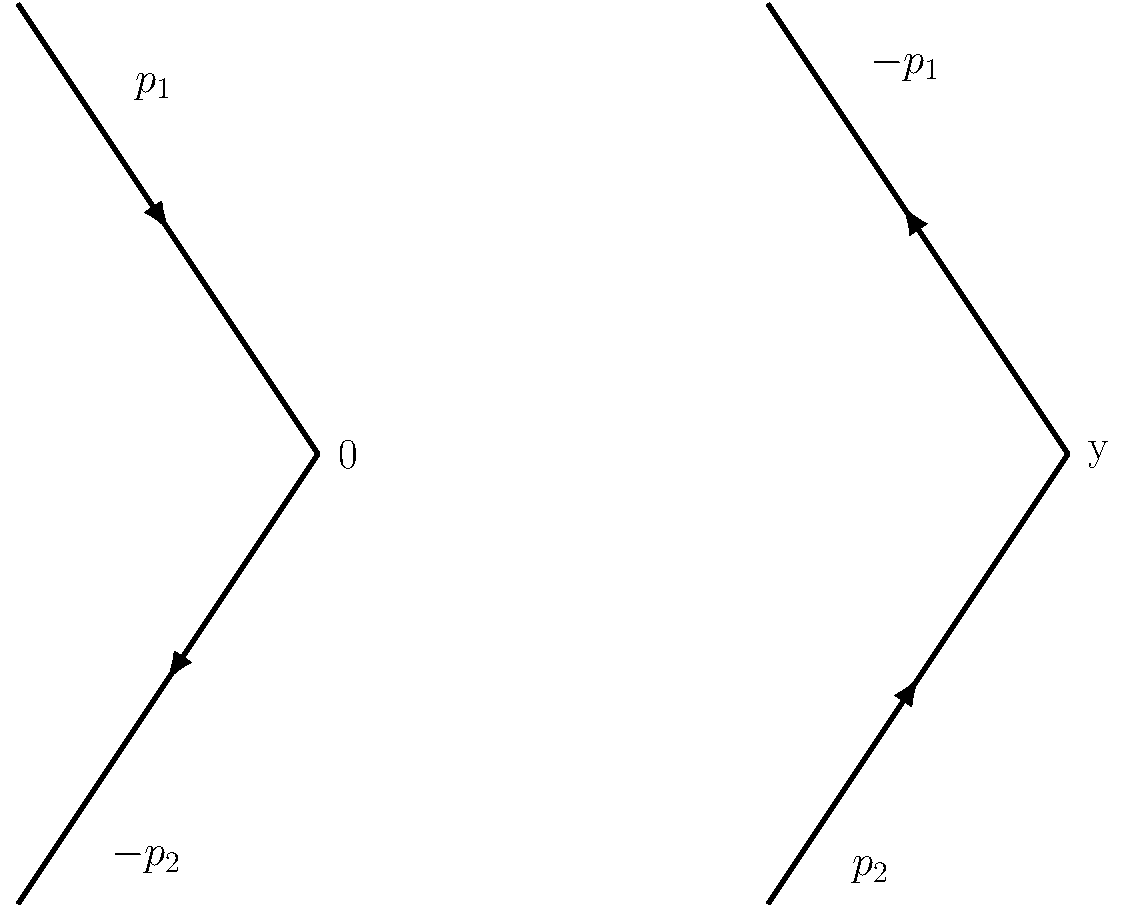
\includegraphics[scale=0.3]{Figures/DrellYanWilsonLoop.pdf}
    \caption{Integration contour for the eikonal approximation in the Drell-Yan process, and $y=(y^{0},\Vec{0})$.}
    \label{fig:DYWilsonLoop}
\end{figure}
%%%%%%%%%%%%%%%%%%%%%%%%%%%%%%%%%%

We can now do the same as we did in \cref{sec:threshold factorization} and use factorization properties of cross sections to define eikonal distributions responsible for the collinear divergences in $\sigma_{ij}^{(\text{eik})}$. 
So the next object to consider is the eikonal analogue to the light-cone distributions $f_{i/i}$. In the limit $x\rightarrow 1$, parton-in-parton distributions can be shown to take the form \cite{Korchemsky:1988si}\footnote{Again, there is an implicit average and sum over colour in the expectation value.}
\begin{align}
    f_{i/i}^{(\text{eik})}(x,\mu,\epsilon)&=\frac{Q}{2}\int_{-\infty}^{\infty}\frac{dy^{-}}{2\pi}\,e^{iy^{-}(1-x)Q/2}\bra{0}\Bar{\mathcal{T}}\{\mathcal{U}_{-p_1}[y,\infty]\}\mathcal{T}\{\mathcal{U}_{p_1}[0,\infty]\}\ket{0}\nonumber
    \\
    &=\frac{Q}{2}\int_{-\infty}^{\infty}\frac{dy^{-}}{2\pi}\,e^{iy^{-}(1-x)Q/2}\mathcal{W}_{\gamma_{p_1}}(y)\,,
\end{align}
where the path $\gamma_{p_1}$ is the $p_1$ part of $\gamma_{DY}$. 

By using these eikonal distributions the eikonal cross section can be written as
\begin{align}\label{eq:1st eikonal cross section}
    \sigma_{ij}^{(\text{eik})}(w,Q,\mu,\alpha_s,\epsilon)&=\int dw_1 dw_2 dw'\,f_{i/i}^{(\text{eik})}(w_1,\mu,\epsilon)\,f_{i/i}^{(\text{eik})}(w_2,\mu,\epsilon)\,\omega_{ij}^{(\text{eik})}(w',Q,\mu,\alpha_s)\nonumber
    \\
    &\hspace{1cm}\delta(w-w_1-w_2-w')\,.
\end{align}
where we defined the energy fractions $w=1-\tau$, $w_1=1-x_1$, $w_2=1-x_2$ and $w'=1-z$. 

In \cref{sec:threshold factorization} we were working in Mellin space, so by taking the Mellin transform of \cref{eq:1st eikonal cross section} we obtain 
\begin{align}\label{eq:eikonal approcximation of partonic}
    \Me{\sigma}^{(\text{eik})}(N,Q,\mu,\alpha_s,\epsilon)=\Me{f}_{i/i}^{(\text{eik})}(N,\mu,\epsilon)\,\Me{f}_{j/j}^{(\text{eik})}(N,\mu,\epsilon)\,\Me{\omega}_{ij}^{(\text{eik})}(N,Q,\mu,\alpha_s)\,,
\end{align}
where we have used that the Mellin transform of the delta function is
\begin{align}
    \int_{0}^{1}d\tau\tau^{N-1}\,\delta(1-\tau-(1-x_1)-(1-x_2)-(1-z))=e^{-N(1-x_1+1-x_2+1-z)}\,,
\end{align}
where $e^{-N(1-x)}=x^{N-1}$ in the large $N$ limit. The result in \cref{eq:eikonal approcximation of partonic} is the eikonal approximation of \cref{eq:partonic analogue to hadronic in mellin }. 

We can also make an eikonal approximation of the near threshold cross section \cref{eq:threshold factorization Mellin}, which can be constructed in a similar fashion as we have done for \cref{eq:eikonal approcximation of partonic}, given by
\begin{align}\label{eq:eikonal approcximation of near threshold}
    \Me{\sigma}^{(\text{eik})}(N,Q,\mu,\alpha_s,\epsilon)=\Me{J}_{i/i}^{(\text{eik})}(N,\mu,\epsilon)\,\Me{J}_{j/j}^{(\text{eik})}(N,\mu,\epsilon)\,\Me{S}_{ij}(N,Q,\mu,\alpha_s)\,,
\end{align}
where we have used that the soft function by definition contains the soft contributions, i.e. $S_{ij}=S_{ij}^{(\text{eik})}$. Then we can use that \cref{eq:eikonal approcximation of partonic} and \cref{eq:eikonal approcximation of near threshold} must be equal near threshold, giving
\begin{align}\label{eq:partonic eikonal with soft function}
    \Me{\omega}_{ij}^{(\text{eik})}(N,Q,\mu,\alpha_s)=\frac{\Me{J}_{i/i}^{(\text{eik})}(N,\mu,\epsilon)\,\Me{J}_{j/j}^{(\text{eik})}(N,\mu,\epsilon)}{\Me{f}_{i/i}^{(\text{eik})}(N,\mu,\epsilon)\,\Me{f}_{j/j}^{(\text{eik})}(N,\mu,\epsilon)}\Me{S}_{ij}(N,Q,\mu,\alpha_s)\,.
\end{align}

Apart from contributions from hard virtual gluons, \cref{eq:partonic eikonal with soft function} is the eikonal approximation of \cref{eq:partonic hard function ratio in mellin}. This means that we have an expression for the soft function $\Me{S}$, so if we solve for the soft function in \cref{eq:partonic eikonal with soft function} and insert it into \cref{eq:partonic hard function ratio in mellin}, we find that the hard partonic function can be written as
\begin{align}\label{eq:partonic and eikonal plus ration}
    \Me{\omega}_{ij}(N,Q,\mu,\alpha_s(\mu))=&\Big[\frac{\Me{J}_{i/i}(N,Q,\epsilon)\Me{J}_{j/j}(N,Q,\epsilon)}{\tilde{f}_{i/i}(N,\mu,\epsilon)\tilde{f}_{j/j}(N,\mu,\epsilon)}\Big]\Big[\frac{\Me{f}_{i/i}^{(\text{eik})}(N,\mu,\epsilon)\,\Me{f}_{j/j}^{(\text{eik})}(N,\mu,\epsilon)}{\Me{J}_{i/i}^{(\text{eik})}(N,\mu,\epsilon)\,\Me{J}_{j/j}^{(\text{eik})}(N,Q,\epsilon)}\Big]\nonumber
    \\
    &H_{ij}(Q,\alpha_{s}(\mu))\,\Me{\omega}_{ij}^{(\text{eik})}(N,Q,\mu,\alpha_s)\,,
\end{align}
where both of these ratios are defined such that they cancel each others collinear divergences. This expression looks daunting, but as previously mentioned the ratios can be simplified by using the renormalization group properties of the distributions, which we will do in \cref{sec:RGE for parton in parton}. The eikonal function $\omega_{ij}^{(\text{eik})}$ is the main function of interest, as it contains the parts where soft contributions cancel to give the large logarithms.

We have managed to bring the hard partonic function $\Me{w}_{ij}$ on a fully factorized form in terms of the eikonal function $\Me{\omega}_{ij}^{(\text{eik})}$. It might not have been obvious what the point of this whole refactorization is, but the idea is that we now have an expression where the IR-divergences are grouped into different terms responsible for different regions of phase space. Before we go into details of how to find the eikonal function $\Me{w}_{ij}
^{\text{(eik)}}$ we will take a closer look at the renormalization properties of Wilson lines and the renormalization group equations for the distributions in \cref{eq:partonic and eikonal plus ration}. The reason for taking this slight detour is to introduce the cusp anomalous dimension, which we will have use for later. %The procedure to calculate it is very complicated, but we will later try to explain how it can be done.

%But first we will in the next couple of sections look at renormalization properties of parton-in-parton distributions in the $x\rightarrow 1$ limit and the renormalization properties of Wilson lines.

\subsection*{Overview of IR-divergences}
We have tried to point out as we went along where the divergences in the different expressions above are, but let us try to make that more clear.

First of all, the hadronic cross section $\sigma_{h_{1}h_{2}}$ is of course finite. On the other hand, we observed in a fixed order calculation at NLO that the partonic function $\omega_{ij}$ has collinear divergences. To single this contribution out we defined a partonic analog to the hadronic cross section \cref{eq:partonic analogue to hadronic in mellin } in Mellin space, in such a way that the parton-in-parton distributions $f_{i/i}$ were responsible for these collinear divergences, rendering $\omega_{ij}$ IR-finite. The consequence of this definition is that the parton-in-hadron distributions $f_{i/h}$ do not contain any singularities, which is important as one wants to take these from experimental measurements. 

From there we went on to write down a near threshold form of the partonic cross section \cref{eq:threshold factorization Mellin}, where all collinear singularities are included in the jet subprocesses $J_{i/i}$. The hard subprocess $H$ includes only lines that are off-shell and does not contain any large logarithms. The soft subprocess $S_{ij}$ is defined to include all wide angle soft radiation.

Finally we made an eikonal cross section $\sigma_{ij}^{(\text{eik})}$ in \cref{eq:eikonal cross section wilson loop}, which contains collinear singularities due to the light-like momenta $p_1$ and $p_2$ of the incoming partons\footnote{Or rather due to the light-like directional vectors $n_{1}$ and $n_{2}$ along the momenta $p_1$ and $p_2$.}. We factorized this cross section in \cref{eq:eikonal approcximation of partonic} and \cref{eq:eikonal approcximation of near threshold} such that $f_{i/i}^{(\text{eik})}$ and $J_{i/i}^{(\text{eik})}$ are responsible for these collinear divergences. The eikonal cross section $\sigma_{ij}
^{(\text{eik})}$ also contains soft divergences, but according to the KLN-theorem these cancel in the sum over all final states, leading to large logarithms. Hence, the soft function $S_{ij}$ and the eikonal function $\omega_{ij}
^{(eik)}$ are free of IR-divergences. 